\documentclass[11.5pt]{article}
\usepackage{stat110}

\title{MGFs and Joint, Conditional, and Marginal Distributions}
\sectionnum{6}

\author{\justin, \creds}

%\SOLUTION

\begin{document}

\maketitle

\begin{notes}

\begin{comment}
\section*{Exponential Distribution (Continuous)}

Let us say that $X$ is distributed $\Expo(\lambda)$. We know the following:
\begin{description}
	\item[Story] You're sitting on an open meadow right before the break of dawn, wishing that airplanes in the night sky were shooting stars, because you could really use a wish right now. You know that shooting stars come on average every 15 minutes, but it's never true that a shooting star is ever "due" to come because you've waited so long. Your waiting time is memorylessness, which means that the time until the next shooting star comes does not depend on how long you've waited already.
	
	\item[Example] The waiting time until the next shooting star is distributed $\Expo(4)$. The 4 here is $\lambda$, or the rate parameter, or how many shooting stars we expect to see in a unit of time. The expected time until the next shooting star is $\frac{1}{\lambda}$, or $\frac{1}{4}$ of an hour. You can expect to wait 15 minutes until the next shooting star.
	
	\item[All Exponentials are Scaled Versions of Each Other]
		\[Y \sim \Expo(\lambda) \rightarrow X = \lambda Y \sim \Expo(1)\]
	 
	\item[PDF and CDF] The PDF and CDF of a Exponential is:
\begin{eqnarray*}
f(x) = \lambda e^{-\lambda x},
\hspace{.1 in}
x \in [0, \infty)
\hspace{1 in}
F(x) = P(X \leq x) = 1 - e^{-\lambda x},
\hspace{.1 in}
x \in [0, \infty)
\end{eqnarray*}
	

	\item[Memorylessness] The Exponential Distribution is the sole continuous memoryless distribution. This means that it's always ``as good as new", which means that the probability of it failing in the next infinitesimal time period is the same as any infinitesimal time period. This means that for an exponentially distributed $X$ and any real numbers $t$ and $s$,
	\[P(X > s + t | X > s) = P(X > t)\]
	Given that you've waited already at least $s$ minutes, the probability of having to wait an additional $t$ minutes is the same as the probability that you have to wait more than $t$ minutes to begin with. Here's another formulation.
	\[X - a | X > a \sim \Expo(\lambda)\]
	Here are two consequences of the memoryless property.
	\begin{enumerate}
		\item If waiting for the bus is distributed exponentially with $\lambda = 6$, no matter how long you've waited so far, the expected additional waiting time until the bus arrives is always $\frac{1}{6}$, or 10 minutes. The distribution of time from now to the arrival is always the same, no matter how long you've waited.
		\item The instantaneous failure rate $\left(\frac{f(x)}{1-F(x)}\right)$, or hazard function, is constant (see \url{http://en.wikipedia.org/wiki/Failure_rate} for more information, or try to think of the hazard function in terms of a conditional probability). That is, if the lifetime of a light bulb is distributed exponentially, the instantaneous rate of failure is always the same - the lightbulb will always have the same probability of failing in the next infinitesimal time unit for the duration of its lifetime. This is unlike real life light bulbs, whose failure rates grow as they grow older or my printer, which fails when I most need it.
	\end{enumerate}
	

\end{description}


\section*{Continuous Distributions}
\begin{center}
\renewcommand{\arraystretch}{3}
\begin{tabular}{cccccc}
\textbf{Distribution} & \textbf{PDF and Support} & \textbf{Expected Value}  & \textbf{Variance}  &\textbf{Equivalent To} & \textbf{MGF}\\
\hline

\shortstack{Uniform \\ \Unif($a, b$)} & \shortstack{$ f(x) = \frac{1}{b-a}, x \in [a, b] $ \\$ f(x) = 0, x \notin [a, b]$} & $\frac{a+b}{2}$ & $\frac{(b-a)^2}{12}$ & $F_X(X)$ ~ & $\frac{e^{tb}-e^{ta}}{t(b-a)}$\\
\hline
\shortstack{Normal \\ $\N(\mu, \sigma^2)$} & $f(x) = \frac{1}{\sigma \sqrt{2\pi}} e^{-\frac{(x - \mu)^2}{2 \sigma^2}}$ & $\mu$  & $\sigma^2$ & ~ & $e^{t\mu + \frac{\sigma^2t^2}{2}}$\\
\hline
\shortstack{Exponential \\ $\Expo(\lambda)$} & \shortstack{$f(x) = \lambda e^{-\lambda y}, x \in [0, \infty)$\\$ f(x) = 0, x \notin [0, \infty)$} & $\sfrac{1}{\lambda}$  & $\sfrac{1}{\lambda^2}$ & ~ & $\frac{\lambda}{\lambda - t}$\\
\hline

\end{tabular}
\end{center}
\end{comment}

\section*{Poisson Process}
The Poisson process gives a story that links the Exponential distribution with the Poisson distribution. A Poisson process with rate $\lambda$ has the following properties:
\begin{enumerate}[label=(\arabic*)]
\item The number of arrivals that occur in an interval of length $t$ is distributed $\Pois(\lambda t)$.
\item The number of arrivals that occur in disjoint intervals are independent of each other.
\end{enumerate}
\begin{figure}[h!]\begin{center}
  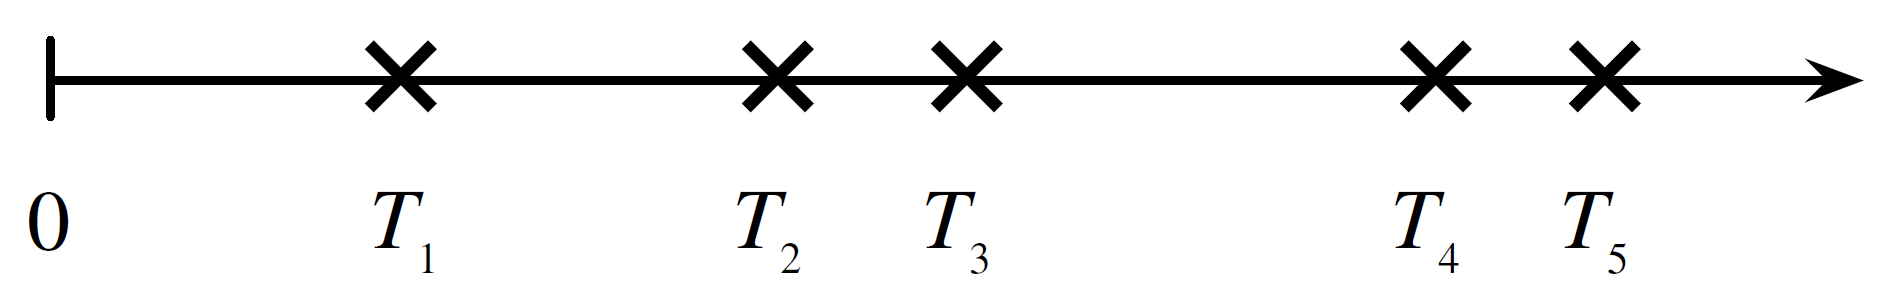
\includegraphics[scale=.4]{poisson_process.png}
  \caption{A Poisson Process. X marks the spot of an arrival. Source - Textbook}
\end{center}\end{figure}

\subsection*{Count-Time Duality}
Instead of asking how many events occur within some amount of time, we can flip the question around and ask how long it takes until some number of events occur. Let $T_n$ be the amount of time it takes until the $n$th event occurs and let $N_t$ be the number of events that occur within time $t$. What relationship do we have between $T_n$ and $N_t$? And what is the intuition behind this 
% Comment this out 
$$P(T_n > t) = P(N_t < n)$$
To reason about this in words, the event that the $n$th arrival time is greater than $t$ is equivalent to the event that the number of arrivals by time $t$ is less than $n$.

Using count-time duality, we can discern the distribution of $T_n$. Let us first look at the distribution for the first arrival. \\
% Comment this out 
For the first arrival, we have
$$P(T_1 \leq t) = 1 - P(T_1 > t) = 1 - P(N_t < 1) = 1 - e^{-\lambda t}$$
This is the $\Expo(\lambda)$ CDF! \\

Now that we know the distribution of $T_1$, what do we know about the distributions of the remaining inter-arrival times?\\

% Comment this out
For $T_2 - T_1$, due to the independence of disjoint intervals, the past is irrelevant once the first arrival occurs, and hence $T_2 - T_1 \sim \Expo(\lambda)$ by the same argument as before. Continuing in this manner, we can argue the same for subsequent inter-arrival times.

\newpage

\section*{Can I Have a Moment?}
\begin{description}
\item[Moment] - Moments describe the shape of a distribution. The first three moments, are related to Mean, Variance, and Skewness of a distribution. The $k^{th}$ moment of a random variable $X$ is
	\[\mu'_k = E(X^k)\]
%\item[Moment about the mean] - The $k^{th}$ moment about the mean of a random variable $X$ is 
%	\[ \mu_k = E[(X-\mu)^k] \]
\item[What's a moment?] Note that 
	\begin{description}
		\item[Mean] $\mu'_1 = E(X)$
		\item[Variance] $\mu'_2 = E(X^2) = Var(X) + (\mu_1')^2$
		%\item[Skewness] $\mu_3 = Skew(X)$
	\end{description}
	Mean, Variance, and other moments (Skewness, Kurtosis, etc.) can be expressed in terms of the moments of a random variable!
\end{description}

\section*{Moment Generating Functions}

\begin{description}
	\item[MGF] For any random variable X, this expected value and function of dummy variable $t$;
		\[ M_X(t) = E(e^{tX}) \]
		is the \textbf{moment generating function (MGF)} of X if it exists for a finitely-sized interval centered around 0. Note that the MGF is just a function of a dummy variable $t$.
	\item[Why is it called the Moment Generating Function?] Because the $k^{th}$ derivative of the moment generating function evaluated 0 is the $k^{th}$ moment of $X$!
	\[\mu_k' = E(X^k) = M_X^{(k)}(0)\]
	Why does this relationship hold? \\
	By differentiation under the integral sign and then plugging in $t=0$
	\begin{align*}
		M_X^{(k)}(t) &= \frac{d^k}{dt^k}E(e^{tX}) = E(\frac{d^k}{dt^k}e^{tX}) = E(X^ke^{tX}) \\
		M_X^{(k)}(0) &= E(X^ke^{0X}) = E(X^k) = \mu_k'
	\end{align*}
	
	\item[MGF of linear combination of X.] If we have $Y = aX + c$, then
		\[M_Y(t) = E(e^{t(aX + c)}) =  e^{ct}E(e^{(at)X}) = e^{ct}M_X(at)\]
		
		
	\item[Uniqueness of the MGF.] \emph{If it exists, the MGF uniquely defines the distribution}. This means that for any two random variables $X$ and $Y$, they are distributed the same (their CDFs/PDFs are equal) if and only if their MGF's are equal. You can't have different PDFs when you have two random variables that have the same MGF.
	\item[Summing Independent R.V.s by Multiplying MGFs.] If $X$ and $Y$ are independent, then
	\begin{align*}
		M_{(X+Y)}(t) &= E(e^{t(X + Y)}) = E(e^{tX}e^{tY}) = E(e^{tX})E(e^{tY}) = M_X(t) \cdot M_Y(t) \\
		M_{(X+Y)}(t) &= M_X(t) \cdot M_Y(t)
	\end{align*}
	The MGF of the sum of two random variables is the product of the MGFs of those two random variables.
\end{description}

\newpage

\section*{Joint Distributions}
Sometimes we have more than one random variable of interest, and we want to study probabilities associated with all of the random variables. Instead of studying the distributions of $X_1, X_2, X_3$ separately, we can study the distribution of the multivariate vector $\textbf{X} = (X_1, X_2, X_3)$. Joint PDFs and CDFs are analogous to multivariate versions of univariate PDFs and CDFs. Usually joint PDFs and PMFs carry more information than the marginal ones do, because they account for the interactions between the various random variables. If, however, the random variables are independent, then the joint PMF/PDF is just the product of the marginals and we get no extra information by studying them jointly rather than marginally.

Joint Probability of events $A$ and $B$: $P(A,B) = P(A \cap B)$

\begin{table}[h]\begin{center}
	\begin{tabular}{ccccc} \toprule
		\textbf{Joint CDF} & ~ & \textbf{Joint PMF} & ~ & \textbf{Joint PDF} \\  \midrule
		$F_{X, Y}(x, y) = P(X \leq x,Y \leq y)$ & ~ & $P(X=x, Y=y)$ & ~ & $f_{X,Y}(x,y) = \frac{\delta}{\delta x} \frac{\delta}{\delta y}F_{X, Y}(x, y)$ \\ \bottomrule
	\end{tabular}\end{center}
\end{table}

Both the Joint PMF and Joint PDF must be non-negative and sum/integrate to 1. ($\sum_x \sum_y P(X=x, Y=y) = 1$) ($\int_x\int_y f_{X,Y}(x,y) = 1$). Like in the univariate case, you sum/integrate the PMF/PDF to get the CDF.

\section*{Conditional Distributions}
By Bayes' Rule, $P(A|B) = \frac{P(B|A)P(A)}{P(B)}$ Similar conditions apply to conditional distributions of random variables.\\

For discrete random variables:
\[P(Y=y|X=x) = \frac{P(X=x, Y=y)}{P(X=x)} = \frac{P(X=x|Y=y)P(Y=y)}{P(X=x)}\]
For continuous random variables:
\[f_{Y|X}(y|x) = \frac{f_{X,Y}(x, y)}{f_X(x)} = \frac{f_{X|Y}(x|y)f_Y(y)}{f_X(x)}\]

\section*{Marginal Distributions}
Law of Total Probability says for an event $A$ and partition $B_1, B_2, ... B_n$: $P(A) = \sum_i P(A\cap B_i)$, which implies that we can find the marginal probability by integrating out the $B$'s.  \\ \\
To find the distribution of one (or more) random variables from a joint distribution, sum or integrate over the irrelevant random variables. \\

Getting the Marginal PMF from the Joint PMF
$$P(X = x) = \sum_y P(X=x, Y=y)$$
Getting the Marginal PDF from the Joint PMF
$$f_X(x) = \int_y f_{X, Y}(x, y) \diff y$$



\section*{Independence of Random Variables}
Review: $A$ and $B$ are independent if and only if either $P(A\cap B) = P(A)P(B)$ or $P(A|B) = P(A)$. \\

Similar conditions apply to determine whether random variables are independent - two random variables are independent if their joint distribution function is simply the product of their marginal distributions, or that the a conditional distribution of is the same as its marginal distribution. \\

In words, random variables $X$ and $Y$ are independent for all $x, y$, if and only if one of the following hold:
\begin{itemize}
	\itemsep -1mm
	\item Joint PMF/PDF/CDFs are the product of the Marginal PMF
	\item Conditional distribution of $X$ given $Y$ is the same as the marginal distribution of $X$
\end{itemize}

\begin{table}[htb]
	\begin{tabular}{ccc}
		$X$ and $Y$ (discrete) are independent  & $\Longleftrightarrow$ & $P(X \leq x, Y \leq y) = P(X \leq x)P(Y \leq y),  \forall x, y$ \\ 
		$X$ and $Y$ (discrete) are independent  & $\Longleftrightarrow$ & $P(X=x, Y=y) = P(X=x)P(Y=y),  \forall x, y$ \\ 
		$X$ and $Y$ (discrete) are independent  & $\Longleftrightarrow$ & $P(X=x | Y=y) = P(X=x),  \forall x, y$ \\ 
		$X$ and $Y$  (continuous) are independent  & $\Longleftrightarrow$ & $P(X \leq x, Y \leq y) = P(X \leq x)P(Y \leq y),  \forall x, y$ \\ 
		$X$ and $Y$  (continuous) are independent  & $\Longleftrightarrow$ & $f_{X, Y}(x, y) = f_X(x)f_Y(y), \forall x, y$ \\ 
		$X$ and $Y$  (continuous) are independent  & $\Longleftrightarrow$ & $f_{X|Y}(X|Y) = f_X(X), \forall x, y$ 
	\end{tabular}
\end{table}

\section*{Multivariate LotUS}
In one dimension, we have: $E(g(X)) = \sum_xg(x)P(X=x)$, or $E(g(X)) = \int_{-\infty}^{\infty}g(x)f_X(x) \diff x$\\ \\ 
For discrete random variables:
$$E(g(X, Y)) = \sum_x\sum_yg(x, y)P(X=x, Y=y)$$
For continuous random variables:
$$E(g(X, Y)) = \int_{-\infty}^{\infty}\int_{-\infty}^{\infty}g(x, y)f_{X,Y}(x, y) \diff x \diff y $$

\end{notes}

\newpage

\section*{Practice Problems} 

\begin{comment}
\begin{exercise}{Simple Memoryless Property} 
Let $X_1$, $X_2$, $X_3$ be independent with $X_i \sim \Expo(\lambda_i)$. Find $E\paren{X_1 + X_2 + X_3 | X_1 > 1, X_2 > 2, X_3 > 3}$ in terms of $\lambda_1, \lambda_2, \lambda_3$
\end{exercise}

\begin{solution}{4} 
Note that $X_1$, $X_2$, and $X_3$ are all independent and that we can use linearity. So we have
\begin{align*}
E\paren{X_1 + X_2 + X_3 | X_1 > 1, X_2 > 2, X_3 > 3} &= E\paren{X_1 | X_1 > 1} + E\paren{X_2 | X_2 > 2} + E\paren{X_3 | X_3 > 3} \\
&= \frac{1}{\lambda_1} + 1 + \frac{1}{\lambda_2} + 2 + \frac{1}{\lambda_3} + 3 \\
&= \frac{1}{\lambda_1} + \frac{1}{\lambda_2} + \frac{1}{\lambda_3} + 6
\end{align*}
\end{solution} 

%%%%%%%%%%%%%%%%%%%%%%%%%%%%%%%%%%%%%%%%%%%%%%%%%%%%%%%%%%%

\begin{exercise}{Time to Failure} 
$n$ lightbulbs are turned on simultaneously. Their lifetimes
are independent Expo($\lambda$) random variables. What is the expected time until all of the lightbulbs
burn out?
\end{exercise}

\begin{solution}{4} 
Let $X_1, X_2, \ldots X_n$ be i.i.d. $\Expo(\lambda)$ representing the amount of time before each of the $n$ lightbulbs burn out. Let $\{T_i\}_{i=1}^{n}$ be the amount to time we must wait between the $i-1$st and $i$th lightbulbs burning out. $T_1 \sim \min(X_1, X_2 \ldots X_n)$ because that the lightbulb with the smallest life expectancy will burn out first. By the minimum of exponentials, we have that $$ T_1 \sim \Expo(\lambda + \lambda + \ldots + \lambda) = \Expo(n \lambda)$$ which means $E(T_1) = \frac{1}{n \lambda}$. 

By a similar argument, we have that $T_2$ is the minimum of $n-1$ of the $X_i$'s, so it has an expected value of $\frac{1}{(n-1)\lambda}$. Therefore, the final answer is: 

$$ E(T) = \sum_{i = 1}^{n} E(T_i) = \frac{1}{\lambda} \left(\frac{1}{n} + \frac{1}{n-1} + \ldots + \frac{1}{2} + \frac{1}{1} \right) $$
\end{solution} 

%%%%%%%%%%%%%%%%%%%%%%%%%%%%%%%%%%%%%%%%%%%%%%%%%%%%%%%%%%%

\begin{exercise}{Emails} 
Emails arrive in an inbox according to a Poisson process with rate $20$ emails per hour. Let $T$ be the time at which the 3rd email arrives, measured in hours after a certain fixed starting time. Find $P(T > 0.1)$ without using calculus.
\end{exercise}

\begin{solution}{3} 
We know that for a Poisson process, the number of emails that arrive in any time interval of size $t$ is distributed $\Pois(\lambda t)$. Consider the first 0.1 hours of this process. The number of emails that arrive during those 0.1 hours is distributed $\Pois(20 \cdot 0.1) = \Pois(2)$. Saying that $T > 0.1$ is the same as saying that the number of emails arriving in the first 0.1 hours is at most 2. Therefore, if $X \sim \Pois(2)$ represents the number of emails you recieve in the first 0.1 hours, then we have: 

$$ P(T > 0.1) = P(X \leq 2) = e^{-2} + \frac{e^{-2}\cdot 2}{1!} + \frac{e^{-2} 2^2}{2!} \approx 0.6767$$
\end{solution} 

%%%%%%%%%%%%%%%%%%%%%%%%%%%%%%%%%%%%%%%%%%%%%%%%%%%%%%%%%%%
\begin{exercise}{Memoryless Post-Office} 
A post offce has 2 clerks. Alice enters the post offce while 2 other customers, Bob and Claire, are being served by the 2 clerks. She is next in line. The amount of time that Bob's clerk takes on each customer is distributed $\Expo(\lambda_1)$, while the amount of time that Alice's clerk takes on each customer is distirbuted $\Expo(\lambda_2)$.  

For this problem, you may use the following fact: If $X \sim \Expo(a)$ and $Y \sim \Expo(b)$, then $P(X < Y) = \frac{a}{a+b}$

\begin{enumerate}
\item What is the probability that Alice is the last of the 3 customers to be done being served?

\item Now, assume that $\lambda_1 = \lambda_2 = \lambda$. What is the expected total time that Alice needs to spend at the post offce?
\end{enumerate}
\end{exercise}

\begin{solution}{4}
Let $B$ be the event that Bob finishes first, and let $C$ be the event that Claire finishes first. 
\begin{enumerate}
\item We use the law of total probability, conditioning on who finishes first. If Bob finishes first, then Claire must finish before Alice. If Claire finishes first, then Bob must finish before Alice. In either case, by the memoryless property, when Alice steps up to the clerk, the distribution of the amount of time that the other person has to wait is the same as before. 

We have: 

\begin{align*}
P(\text{Alice last}) &= P(\text{Claire finishes before Alice} | B) P(B) \\ &+ P(\text{Bob finishes before Alice} |  A) \cdot P(A) \\ 
&= \frac{\lambda_2}{\lambda_1 + \lambda_2} \cdot \frac{\lambda_1}{\lambda_1+\lambda_2} +\frac{\lambda_1}{\lambda1+\lambda_2}\cdot \frac{\lambda_2}{\lambda_1 + \lambda_2} \\ 
&= \frac{2 \lambda_1 \lambda_2}{(\lambda_1 + \lambda_2)^2}
\end{align*}
\item The amount of time Alice waits in line is the miniumum of 2 exponentials, so it is distributed $\Expo(2 \lambda)$. Then, once she gets to a clerk, her waiting time is $\Expo(\lambda)$. Therefore, the expected total amount of time she spends in the post office is: 

$$ \frac{1}{2 \lambda} + \frac{1}{\lambda} = \frac{3}{2 \lambda}$$
\end{enumerate}
\end{solution}
\end{comment}

\begin{exercise}{Procrastinators}
Three students are working independently on their Stat 110 problem set. All three start at 1pm on the day the pset is due, and each takes an Exponential time with mean 6 hours to complete the homework. What is the earliest time when all three students will have completed the homework, on average? 
\end{exercise}

\begin{solution}{2}
Label the students, and let $X_i$ be the amount of time it takes student $i$ to finish the pset. Let $T$ be the total amount of time it takes for all three students to finish, and let $T = T_1 + T_2 + T_3$, where $T_1 = \min(X_1, X_2,X_3)$, and so on. We know that $T_1 \sim \Expo(\frac{3}{6})$, as we showed in the previous problem set, $T_2 \sim \Expo(\frac{2}{6})$, and $T_3\sim \Expo(\frac{1}{6})$. Therefore, $E[T] = 2 + 3 + 6 =11$
\end{solution}

\begin{exercise}{Counting Cars}
Cars pass by a certain point on a road according to a Poisson process with rate $\lambda$ cars/minute. Let $N_t \sim \Pois(\lambda t)$ be the number of cars that pass by that point in the time interval $[0, t]$, with $t$ measured in minutes.
\begin{enumerate}
\item A certain device is able to count cars as they pass by, but it does not record the arrival times. At time 0, the counter on the device is reset to 0. At time 3 minutes, the device is observed and it is found that exactly 1 car had passed by. Given this information, find the conditional CDF of when that car arrived. Also describe in words what the result says.

\item In the late afternoon, you are counting blue cars. Each car that passes by is blue with probability $b$, independently of all other cars. Find the joint PMF and marginal PMFs of the number of blue cars and number of non-blue cars that pass by the point in 10 minutes.
\end{enumerate}
\end{exercise}

\begin{solution}{3.5}
\vspace{-5mm}
\begin{enumerate}
    \item Let $T_1$ be the arrival time of the first car to arrive after time 0. Unconditionally, $T_1 \sim \Expo(\lambda)$. Given $N_3 = 1$, for $0 \leq t \leq 3$, we have
    $$P(T_1 \leq t | N_3 = 1) = P(N_t \geq 1 | N_3 = 1) = \frac{P(N_t \geq 1, N_3 = 1)}{P(N_3 = 1)} = \frac{P(N_t = 1, N_3 = 1)}{P(N_3 = 1)}$$
    By definition of the Poisson process, the numerator is
    $$P(N_t = 1, N_3 = 1) = P\paren{N_{[0, t]} = 1, N_{(t, 3]} = 0} = P\paren{N_{[0, t]} = 1}P\paren{N_{(t, 3]} = 0} = e^{-\lambda t}\lambda t e^{-\lambda(3 - t)} = \lambda t e^{-3 \lambda}$$
    and the denominator is $e^{-3\lambda} 3 \lambda$. Hence,
    $$P(T_1 \leq t | N_3 = 1) = \frac{\lambda t e^{-3 \lambda}}{e^{-3\lambda} 3 \lambda} = \frac{t}{3}$$
    for $0 \leq t \leq 3$ (and 0 for $t < 0$ and 1 for $t > 3$). \\
    This says that the conditional distribution of the first arrival time, given that there was exactly one arrival in $[0, 3]$, is $\Unif(0, 3)$.
    \item Let $X$ and $Y$ be the number of blue and non-blue cars that pass by in those 10 minutes respectively, and $N = X + Y$. Then $N \sim \Pois(10\lambda)$ and $X|N \sim \Bin(N, b)$. By the chicken-egg story, $X$ and $Y$ are independent with $X \sim \Pois(10 \lambda b)$, $Y \sim \Pois(10 \lambda (1 - b))$. The joint PMF is the product of the marginal PMFs:
    $$P(X = x, Y = y) = \frac{e^{-10 \lambda b}(10 \lambda b)^x}{x!}\frac{e^{-10 \lambda (1 - b)}(10 \lambda (1 - b))^y}{y!}$$
    for all nonnegative integers $x, y$.
\end{enumerate}
\end{solution}

\begin{exercise}{Linear Combination of Independent Normals} 
Let $X_1 \sim \N(\mu_1, \sigma_1^2)$ and $X_2 \sim \N(\mu_2, \sigma_2^2)$. Use the MGF to show that for any values of $a, b \not= 0$, $Y = a X_1 + b X_2$ is also Normal. (You may use the fact that the MGF of a $\N(\mu, \sigma^2)$ distribution is $e^{\mu t + \frac{1}{2}\sigma^2 t^2}$.)  
\end{exercise}

\begin{solution}{4} 
We know that the MGF for the sum of 2 independent random variables is the product of their individual MGFs. We also know that the MGF of a scalar $c$ times a random variable is equal to that random variable's MGF with $ct$ subsituted for $t$. 

\begin{align*}
M_Y(t) &= \exp \left(\mu_1 (at) + \frac{1}{2} \sigma_1^2 (at)^2\right) \cdot \exp\left(\mu_2 (bt) + \frac{1}{2} \sigma_2^2 (bt)^2\right) \\ 
&=
\exp\left( \mu_1 (at) + \frac{1}{2} \sigma_1^2 (at)^2 + \mu_2 (bt) + \frac{1}{2} \sigma_2^2 (bt)^2\right) \\ 
&= \exp\left( (a\mu_1 + b \mu_2)t  + \paren{\frac{(a \sigma_1)^2 + (b \sigma_2)^2}{2} } t^2\right) 
\end{align*}

This is the $\N\paren{a \mu_1 + b \mu_2, a^2 \sigma_1^2 + b^2 \sigma_2^2}$ MGF.
\end{solution} 

%%%%%%%%%%%%%%%%%%%%%%%%%%%%%%%%%%%%%%%%%%%%%%%%%%%%%%%%%%%
\begin{exercise}{Return of Nick and Hibbert}
One of two doctors, Dr. Hibbert and Dr. Nick, is called upon to perform a series of $n$ surgeries. Let $H$ be the indicator random variable for Dr. Hibbert performing the surgeries, and suppose that $E(H) = p$. Given tht Dr. Hibbert is performing the surgeries, each surgery is successful with probability $a$, independently. Given that Dr. Nick is performing the surgeries, each surgery is successful with probability $b$ independently. Let $X$ be the number of successful surgeries. 

\begin{enumerate}
    \item Find the joint PMF of $H$ and $X$.
    \item Find the marginal PMF of $X$. 
    \item Find the conditional PMF of $H$ given $X=k$. 
\end{enumerate}
\end{exercise}

\begin{solution}{4}
\begin{enumerate}
    \item We find the joint PMF by recalling the definition of conditional probability. 
    $$P(X = x | H=h) = \frac{P(H=h, X=x)}{P(H=h)}\implies P(H=h, X=x) = P(X=x|H=h)P(H=h)$$
    From here, we use the fact that $H$ can only take on two values and define a piecewise function. 
    $$ 
    P(X=x|H=h)P(H=h) = \begin{cases}
    {n \choose x}a^x(1-a)^{n-x}p, \text { if } h =1\\
    {n \choose x}b^x(1-b)^{n-x}(1-p) \text{ if } h = 0 
    \end{cases}
    $$
    \item To find the marginal PMF of $X$, we must eliminate $H$ from the joint PMF. To do so, we sum over all possible values of $H$. 
    $$P(X=x) = 
    P(H=1, X=x) + P(H=0, X=x) 
    $$
    where we plug in our piecewise function from above. 
    \item The conditional PMF is found using the definition of conditional probability. 
    $$P(H=h | X=x)  = \frac{P(H=h, X=x)}{P(X=x)}
    $$
    where the joint PMF is defined as above. 
\end{enumerate}
\end{solution}
%%%%%%%%%%%%%%%%%%%%%%%%%%%%%%%%%%%%%%%%%%%%%%%%%%%%%%%%%%%

\begin{exercise}{Probabilities Using Joint CDFs and PDFs}
Let $X$ and $Y$ be continuous random variables. What is the probability that $(X, Y)$ falls into the 2-D rectangle $[a_1, a_2] \times [b_1, b_2]$ in terms of a) the joint CDF of $X$ and $Y$, $F(x, y)$, and b) the joint PDF of $x$ and $Y$, $f(x, y)$?
\end{exercise}

\begin{solution}{4}
\vspace{-5mm}
\begin{enumerate}
\item $F(a_2, b_2) - F(a_1, b_2) - F(a_2, b_1) + F(a_1, b_1)$. Draw a picture to see this.
\item We can integrate the joint PDF over the region of interest to get the probability:
$$P\paren{(X, Y) \in [a_1, a_2] \times [b_1, b_2]} = \int_{b_1}^{b_2} \int_{a_1}^{a_2} f(x, y) \diff x \diff y$$
\end{enumerate}
\end{solution}

\begin{exercise}{LogNormal Moments} 
Let $Z \sim \N(0, 1)$ and $Y = e^Z$. Then $Y$ has a LogNormal distribution (because its log is Normal!).
\begin{enumerate}
\item Find \textbf{all} the moments of $Y$. That is, find $E(Y^n)$ for all $n$. 
\item Show the MGF of $Y$ does not exist, by arguing that the integral $E\paren{e^{tY}}$ diverges for $t > 0$.
\end{enumerate}
\end{exercise}

\begin{solution}{4}
\vspace{-5mm}
\begin{enumerate}
\item 
$$E\paren{Y^n} = E\paren{\paren{e^Z}^n} = E\paren{e^{nZ}}$$
We may be tempted to use LOTUS at this point, but it is easier to recognize that $E\paren{e^{nZ}}$ is the MGF of $Z$, evaluated at $t = n$. In other words, $E\paren{e^{nZ}} = M_Z(n)$. Since $M_Z(t) = e^{t^2/2}$, we conclude that $M_Z(n) = e^{n^2/2}$.
\item
$$E\paren{e^{tY}} = E\paren{e^{te^Z}} = \int_{-\infty}^\infty e^{te^z} \frac{1}{\sqrt{2 \pi}} e^{-z^2/2} \textrm{d} z = \int_{-\infty}^\infty \frac{1}{\sqrt{2 \pi}} e^{te^z -z^2/2} \textrm{d} z$$
Suppose $t > 0$. Then as $z$ grows larger, $te^z$ will grow at a faster rate than $z^2 / 2$. Hence, $te^z - z^2 / 2$ will explode. Therefore, the integral diverges for all $t > 0$. Since $E\paren{e^{tY}}$ is not finite on an open interval around 0, the MGF of $Y$ does not exist.
\end{enumerate}
\end{solution} 


%%%%%%%%%%%%%%%%%%%%%%%%%%%%%%%%%%%%%%%%%%%%%%%%%%%%%%%%%%%
\begin{comment}
\begin{exercise}{Discrete max and min} 
Let $X$ and $Y$ be i.i.d. $\Pois(\lambda)$, $L = \min(X, Y)$, and $M = \max(X, Y)$. Find the joint PMF of $L$ and $M$. Are $L$ and $M$ independent?
\end{exercise} 

\begin{solution}{3} 
We want $P(L = l, M = m)$ for all pairs $(l, m)$. Let's consider the three cases.
\begin{enumerate}[label=\arabic*.]
\item $l > m$: $P(L = l, M = m) = 0$
\item $l < m$:
\begin{align*}
P(L = l, M = m) &= P(X = l, Y = m) + P(X = m, Y = l) \\
&= 2 P(X = l, Y = m) & \textrm{by symmetry} \\
&= 2 P(X = l) P(Y = m) & \textrm{by independence of $X$ and $Y$} \\
&= 2 \frac{e^{-\lambda} \lambda^l}{l!} \frac{e^{-\lambda} \lambda^m}{m!}
\end{align*}
\item $l = m$:
\begin{align*}
P(L = l, M = m) &= P(L = l, M = l) \\
&= P(X = l, Y = l) \\
&= \paren{\frac{e^{-\lambda} \lambda^l}{l!}}^2
\end{align*}
\end{enumerate}
This fully specifies the joint PMF of $L$ and $M$. No, $L$ and $M$ are not independent. Knowning the value of $L$ constrains the possible values of $M$ and vice versa.
\end{solution}

%%%%%%%%%%%%%%%%%%%%%%%%%%%%%%%%%%%%%%%%%%%%%%%%%%%%%%%%%%%

\begin{exercise}{A Tale of Two Exponentials}
Let $X$ and $Y$ be continuous positive random variables.
\begin{enumerate}
\item Express $P(X < Y)$ in terms of the joint PDF of $X, Y$. 
\item Let's say that independently, $X \sim \Expo(\lambda_1)$ and $Y \sim \Expo(\lambda_2)$. What is the joint PDF of X, Y?
\item What is $P(X < Y)$?	
\end{enumerate}
\end{exercise}

\begin{solution}{4}
\vspace{-5mm}
\begin{enumerate}
\item To find probabilities, we want to integrate over the joint density over the possible values of $x, y$ that we are interested in. In this case, $Y$ can be any number $y \in [0, 1)$ , and $X | Y = y$ can be any number $x \in [0, y)$. We do a double integral over these regions.
$$P(X < Y) = \int_0^\infty \int_0^y f(x, y) \, dx \, dy$$
\item Let $f(x)$ be the PDF of $X$ and $g(x)$ be the PDF of $Y$. Because they are independent, we have that the joint PDF is simply the product of the marginal PDFs.
$$f(x, y) = f_X(x)f_Y(y) = \lambda_1 e^{-\lambda_1 x} \lambda_2 e^{-\lambda_2 y}$$
\item Combining the results from the first two parts, we have
\begin{align*}
P(X < Y) &= \int_0^\infty \int_0^y f(x, y) \, dx \, dy \\
&= \int_0^\infty \int_0^y f_X(x) f_Y(y) \, dx \, dy \\
&= \int_0^\infty f_Y(y) \int_0^y f_X(x) \, dx \, dy \\
&= \int_0^\infty f_Y(y) \brack{\int_0^y f_X(x) \, dx} \, dy \\
&= \int_0^\infty f_Y(y) F_X(y) \, dy \\
\end{align*}
Now we can plug in values and solve, noting the facts that PDFs must integrate to 1.
\begin{align*}
&= \int_0^\infty \lambda_2 e^{-\lambda_2 y} \paren{1 - e^{-\lambda_1 y}} \, dy \\
&= \int_0^\infty \lambda_2 e^{-\lambda_2 y} \, dy - \int_0^\infty \lambda_2 e^{-\lambda_2 y} e^{-\lambda_1 y} \, dy \\
&= \int_0^\infty \lambda_2 e^{-\lambda_2 y} \, dy - \int_0^\infty \lambda_2 e^{-(\lambda_1 + \lambda_2) y} \, dy \\
&= 1 - \frac{\lambda_2}{\lambda_1 + \lambda_2} \int_0^\infty (\lambda_1 + \lambda_2) e^{-(\lambda_1 + \lambda_2) y} \, dy \\
&= 1 - \frac{\lambda_2}{\lambda_1 + \lambda_2} \\
&= \frac{\lambda_1}{\lambda_1 + \lambda_2} \\
\end{align*}
\end{enumerate}
\end{solution}
\end{comment}
%%%%%%%%%%%%%%%%%%%%%%%%%%%%%%%%%%%%%%%%%%%%%%%%%%%%%%%%%%%

\end{document}
